% !TEX root = ANA-GENR-2018-01-INT1.tex
% Turn off some chktex warnings.
% chktex-file 1 chktex-file 8 chktex-file 46

%------------------------------------------------------------------------------
\section{Author Lists, Acknowledgements and the Proofs Checker}%
\label{sec:Authorlists_Acknowledgements_and_ProofChecker}
%------------------------------------------------------------------------------

%------------------------------------------------------------------------------
\subsection{Author lists and Acknowledgments files}%
\label{sec:Author_lists_and_acknowledgments_files}

\GSnote{}{This feels sliiiiightly similar to \cref{sec:Authorlists_acknowledgments_and_ProofChecker} and perhaps combining the two will be helpful somehow...}

Both types of \GSnote{files}{Not types, but categories. These files are JSON type files, no?}, the author list and the acknowledgements, are built using the FENCE framework, see \cref{fig:authorlist_interface},
and automatically pushed to the appropriate Gitlab repository, using the FENCE--\gitlab integration (\cref{sec:FENCE-Gitlab_Integration}).
Their integration into the paper is straightforward for a \GSnote{future submission to a journal}{Not everything is submitted to a journal, what about CONF and PUB?}.
FENCE provides an elegant way to retrieve the required information from the database (see \cref{sec:MBF_Models_Builder_and_Factories_infrastructure}) and build all the files.

The author list \GSnote{XML file}{First time mentioning XML. Why XML when everything else was JSON?} is composed of three main blocks:
\begin{itemize}
\item Header: store paper main information (\cref{app:author:xmlheader})
\item Institutes: list of institutes and their references (\cref{app:author:xmlinstitute})
\item Authors: list of authors for this author list with their information (\cref{app:author:xmlauthor})
\end{itemize}

The XML file is the one used as a \enquote{role}, since it contains all the information needed to build the other files.
It is the first one to be generated and a backup version of the first release of the author list is stored.

The acknowledgment \File{tex} file is built using a standard template and is filled using the FENCE framework to retrieve the required information about the ATLAS Funding Agencies.

\begin{figure}[htb]
  \centering
  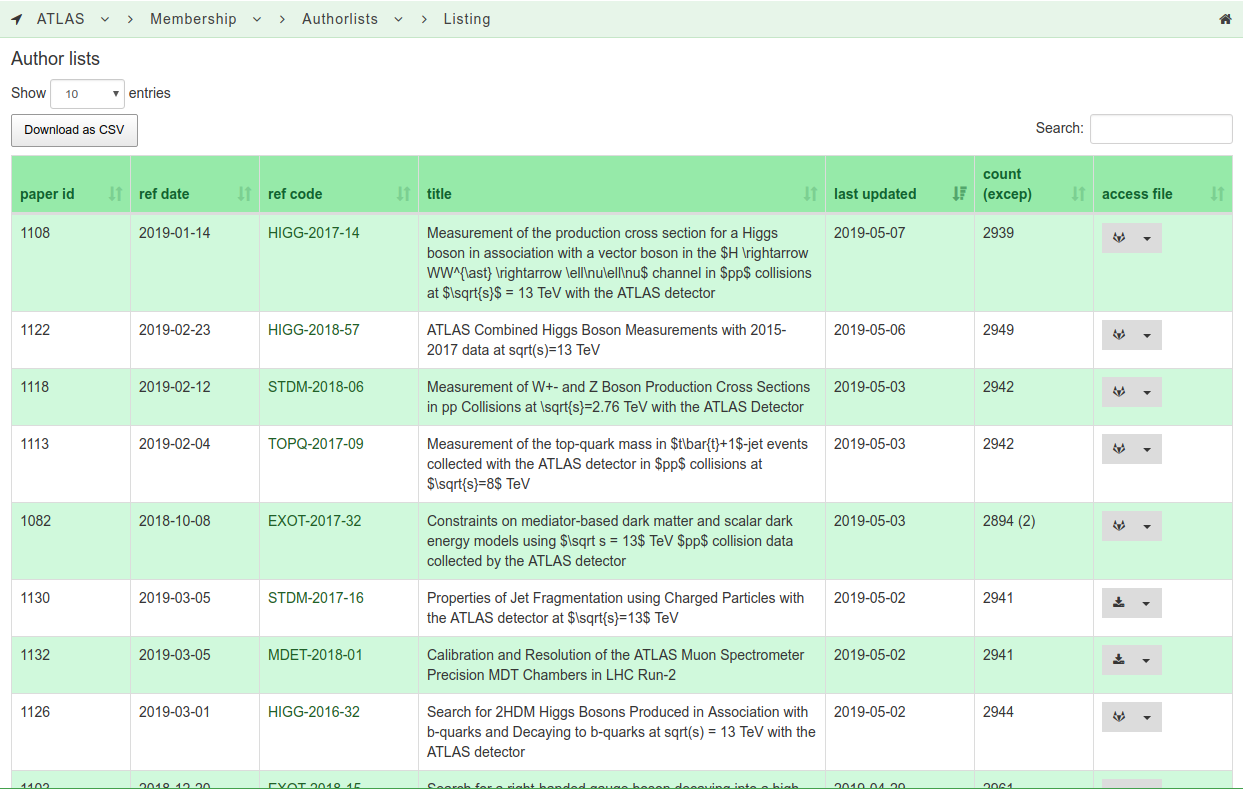
\includegraphics[width=0.9\textwidth]{figures/authorlist_interface.png}%
  \caption{FENCE author list interface.
    The first five entries in the list are GitLab projects.
    \GSnote[inline]{}{They're not all gitlab projects? Just crop this to show only the first five then. I'm confused here. Expand this caption more too.}}%
  \label{fig:authorlist_interface}
\end{figure}

%------------------------------------------------------------------------------
\subsection{Main functionalities of the FENCE Author list user interface}
\label{sec:Main_functionalities_of_the_FENCE_Author_list_user_interface}

The FENCE author list interface, \cref{fig:authorlist_interface}, shows the complete set of author lists created for each ATLAS paper that has been published since 2009 or is being submitted.
They are easily filtered using the SEARCH box option.
All the columns are self-explanatory; in the last column the dropdown menu gives access to the author list location, which can be distinguished by the icon:
a download icon (\GSnote{\faDownload}{Please make FontAwesome part of the detail ATLAS latex. Please. This is probably more for Ian, but ok.}) means the files are stored in AFS and can be downloaded.
A GitLab icon (\faGitlab) means the Paper and the files are located in a PO Gitlab repository. The author lists can be downloaded or displayed in GitLab in different file formats (\GSnote{\File{tex, xml, csv, pdf, cds}}{What's the CDS file format?}) and structures (by country/institutes, or institutes only).

%------------------------------------------------------------------------------
\subsection{Proof checker functionalities}
\label{sec:Proof_checker_functionalities}

Once the author list is sent to the journal together with the publication,
it is time to check if the publisher correctly used the information provided by going through the journal \GSnote{PDFF}{PDF} file sent to ATLAS Physics Office and comparing it to the \File{xml/tex} file.
This process, which used to be done by hand, required the officer to verify if each author ($\sim$2800) and each institute ($\sim$200) is correctly reported and matched.
For this purpose, a tool, the proof checker, was created to automatically poll the proof directories for new PDF documents uploaded.
If it finds a document that has not been checked before, it starts the following process:

\begin{itemize}
\item retrieve the information from the \GSnote{XML file}{Which XML file} created on Paper Submission Phase;
\item extract the text from the journal PDF file;
\item parse the text from the PDF file, creating the target reference;
\item compare the official reference obtained from the XML file with the target reference;
\item create a report with the differences found between the original and the target reference;
\item link the report to the main report page, \cref{fig:collaboration_proofs}.
\end{itemize}

\begin{figure}[htb]
  \centering
  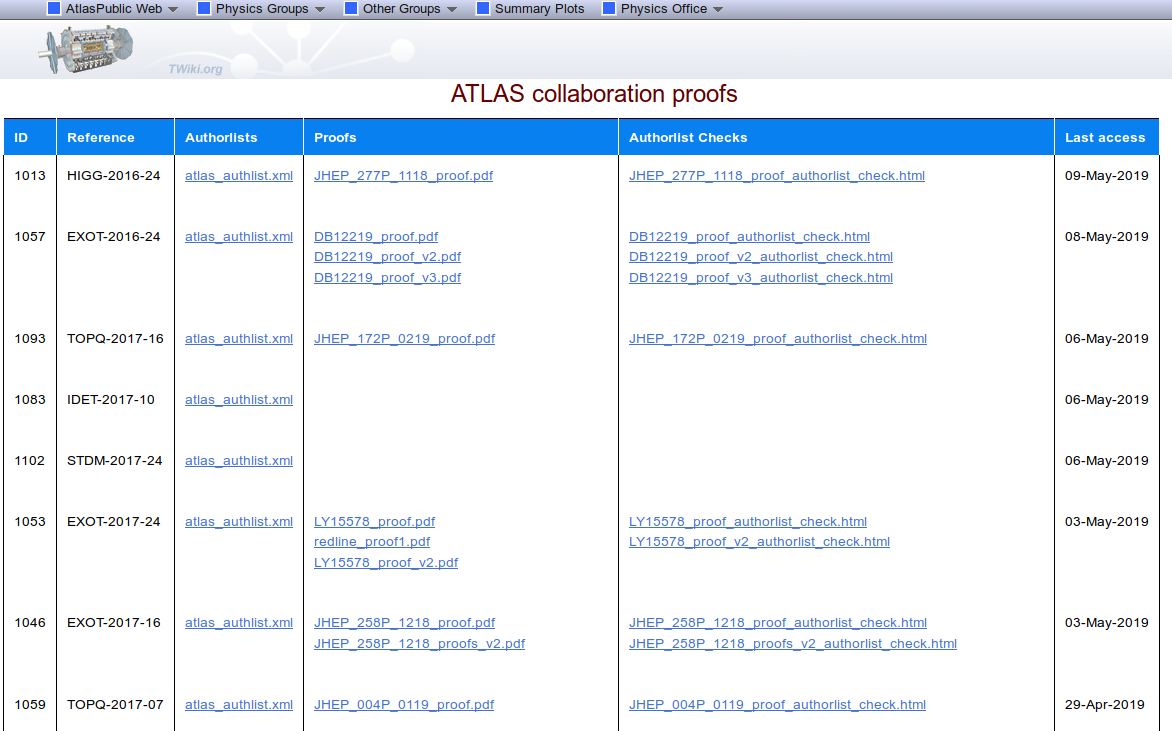
\includegraphics[width=0.9\textwidth]{collaboration_proofs}
  \caption{ATLAS collaboration proofs main page.
    \GSnote[inline]{}{Please expand caption with more detail... e.g. what are the columns?}}
  \label{fig:collaboration_proofs}
\end{figure}

\GSnote{}{What does an example good proof and bad proof look like?}

The main difficulties in this process rely on extracting the content from the PDF file; the text is not easily retrieved for different reasons.
One is that there are a lot of elements that have to be identified and ignored, such as row numbers, watermarks, footers and headings.
Another reason is that words extracted from a PDF file don't follow a specific coding convention:
it can contain non-ASCII characters that can be output in many different ways;
the PDF file can specify a predefined encoding to use, or provide a lookup table of differences between a predefined and a built-in encoding;
for fonts with non-common Latin characters, which is always the case for these kind of publications and content,
special encodings are used and it is necessary to provide a ToUnicode table where semantic information about the characters has to be preserved.
Also the proof checker has to pass through all the publication text and try to \enquote{understand} where the author list starts, where it ends, where the institute list starts and when it ends.
All this is made even more difficult due to the fact that different publishers have different layouts, and create different versions of PDF files.
This makes all of the above problems not generic,
but often specific to a particular publisher.

After the target reference is created, the comparison looks for:
\begin{itemize}
\item authors that seem to be missing from the PDF. Here, false positives are often due to characters encoding and spaces;
\item authors with inconsistent punctuation. This section points out differences between original and target references authors's first names punctuation,
which can follow the rules X. or X.Y. or X.-Y. or X-Y. with or without space;
\item institutes that seem missing from the PDF. Here false positives are often due to non-standard characters that breaks the entry;
\item institutes with close matches. All the entries that really look like the original but have some inconsistencies land in this group.
  Some publishers expand(or contract) USA to United States of America,
  or there is a new character that does not break the institute entry,
  but makes it so that the match is not perfect match, such as \enquote{Università} and \enquote{Universit` a};
\item Mismatched authors. All the authors collaborate through one or more institutes.
  It is checked that the link between the author and the institute is consistent.
  This sometimes results in a false positive,
  because it is not always easy to extract from the PDF file the index number of an institute,
  mainly because the text coming from the PDF file is often full of other elements such as line numbers of the document.
  For this reason an author originally assigned to institute number X, can result matched with target institute YX,
  because in the text extracted from the pdf the number X might be preceded by a Y line number;
  institute YX mostly doesn’t exist or eventually comes to be another institute;
\item Deceased authors. In two categories we show a list, often empty, of authors that we signed as deceased but the publication forgot to mark, or vice-versa.
  The results here are pretty reliable;
\item Missing funding agencies, or wrongly added by the publisher are checked.
\end{itemize}

In early 2019, due to some changes on CERN systems, the component written in PROLOG which ran the comparison went out of service.
This implied an urgent request for developing a new tool that could take care of this task.
PROLOG is well known to take a different approach in a generic problem solving situation,
where the expression of the problem is translated in a logic way instead of working directly on its resolution algorithm.
However, PROLOG is a language that is difficult to maintain,
due to the fact that not many developers had ever a chance to work with it and its logic programming paradigm.
Hence Python was chosen to accomplish this role.

The main issue was to find a way to get the best match among all the items of an array of institutes and authors,
because we cannot blindly rely on finding an author or institute in the same position of the sequence.
It is therefore not possible to just compare \texttt{author~1} in the xml file with \texttt{author~1} in the pdf file and so on.
For this purpose the concept of Levenshtein distance (\cref{app:proofs:levenshtein}) has been used,
so that a weighted index of similarity can be obtained to \enquote{decide} what is matched with what, and to then effectively start checking for anomalies.

At the end, a feature was developed to help the script to evaluate as perfect matches some that wouldn’t otherwise.
A list of \enquote{synonyms} is created for every entry, author or institute,
to teach the proof checker to validate similar strings when the differences are due only to problems we have when decoding the text from the PDF file.
So, for instance, if author \textbf{A. Filipčič} is not found in the target reference,
but from the PDF entries we extracted an author with name \textbf{A. FilipÅŸ ciÅŸ c}, then,
as it has been previously verified that in the PDF file the name appears as expected, the proof checker considers it a perfect match, and skips the problem.
A very long list of false positives can be found in the report page as \enquote{skipped items}.
The list of synonyms is updated manually, but a tool, the Synonym webpage (\cref{sec:Synonym_webpage}), has been created to allow users to update this list themselves.


%------------------------------------------------------------------------------
\subsubsection{Proof checker synonyms}%
\label{sec:Proof_checker_synonyms}

The comparison between PDF file (coming from the Journals) and the XML file (provided by FENCE author list interface) generates a lot of false positives as described in \cref{sec:Report_page}:
special characters encoding can be different, countries sometimes are spelled differently, etc.
To avoid having a huge list of these kind of false positives in the report page that can confuse the users, the new version of the proof checker includes a \enquote{synonyms} list that allows the comparison script to understand if the difference is a real error or another correct way to display the same information.
\IBnote{}{Isn't this a repeat of the above?}
An example of a working synonym is:
\begin{table}[htb]
  \centering
  \begin{tabular}{c}
  \textbf{Institute as stored into ATLAS DB \& XML file} \\
  Physics Department, SUNY Albany, Albany NY, United States of America \\
  \midrule
  \textbf{Institute as written on the journal's author list} \\
  Physics Department, SUNY Albany, Albany, New York, USA
  \end{tabular}
\end{table}

These differences are acceptable, since the main information is correctly displayed and no real errors are found.

All the synonym records are managed using a JSON file and split by institutes and authors (\cref{app:proofs:institute,app:proofs:author}).
Having this as a JSON file allows the proof checker script to easily parse the records and understand if the faults must be marked as journal errors or if they should be skipped.

%------------------------------------------------------------------------------
\subsubsection{Synonym webpage}
\label{sec:Synonym_webpage}

To manage the list of proofs checker synonyms ATLAS PO provides a webpage that allows users to search for an existing entry and manage the record synonyms.
Searching for an institute, or author, will display the list of records that match the searching criteria (\cref{fig:synonym_webpage}) and allows the users to edit the synonyms for the record.
Clicking the edit icon shows a new page section where users can insert their own known synonym for the record.
After confirmation, this will be added to the list of synonyms and will be taken into account by the next run of the proofs checker.

\begin{figure}[htb]
  \centering
  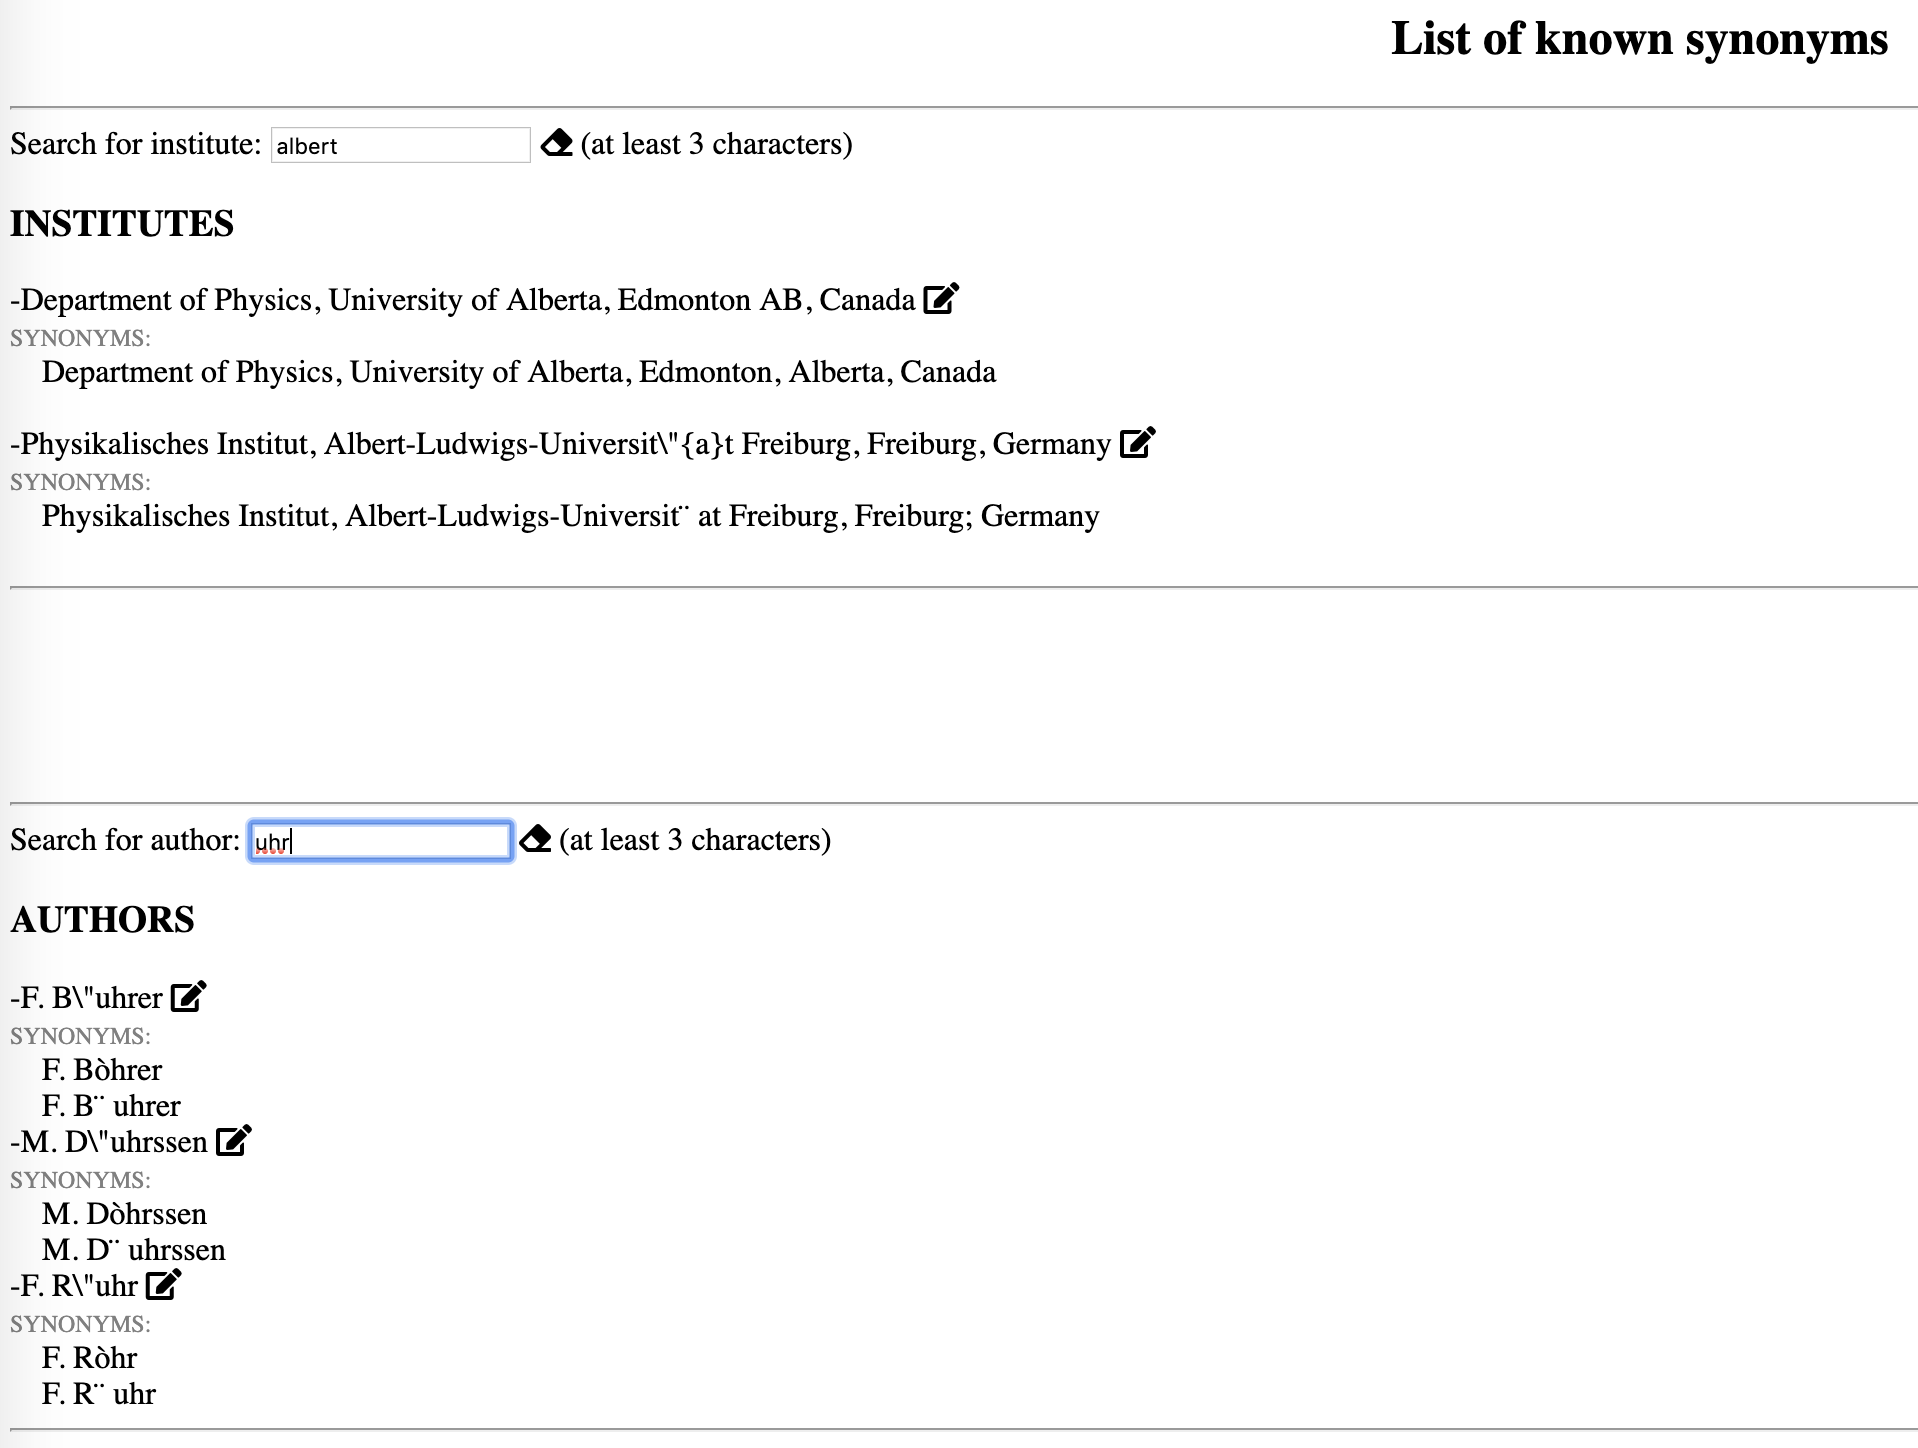
\includegraphics[width=0.9\textwidth]{synonym_webpage}
  \caption{Proof checker synonyms webpage.}
  \label{fig:synonym_webpage}
\end{figure}

%------------------------------------------------------------------------------
\subsubsection{Report page}
\label{sec:Report_page}

The proofs checker provides a report after its run, one for each paper and draft version.
This report is provided and stored in a JSON file and must be parsed to show the report results in a human readable way.
This is done by the \texttt{proof\_report} webpage (\cref{fig:proof_report_webpage}).
The report contains all the paper information plus the real comparison results split by issue sections (see \cref{app:proofs:report}).
The JSON file contains more information than that which is displayed;
this is done to allow the webpage to understand the correct way to show the huge amount of information and for future improvements.
The webpage contains some \enquote{hidden} sections that are produced by the proof checker thanks to the known synonyms,
and can be displayed by clicking on \enquote{Skipped +}.
Here the page will show all the false positive results that the proofs checker found on its comparison, but that are ignored thanks to the synonyms.

\begin{figure}[htb]
  \centering
  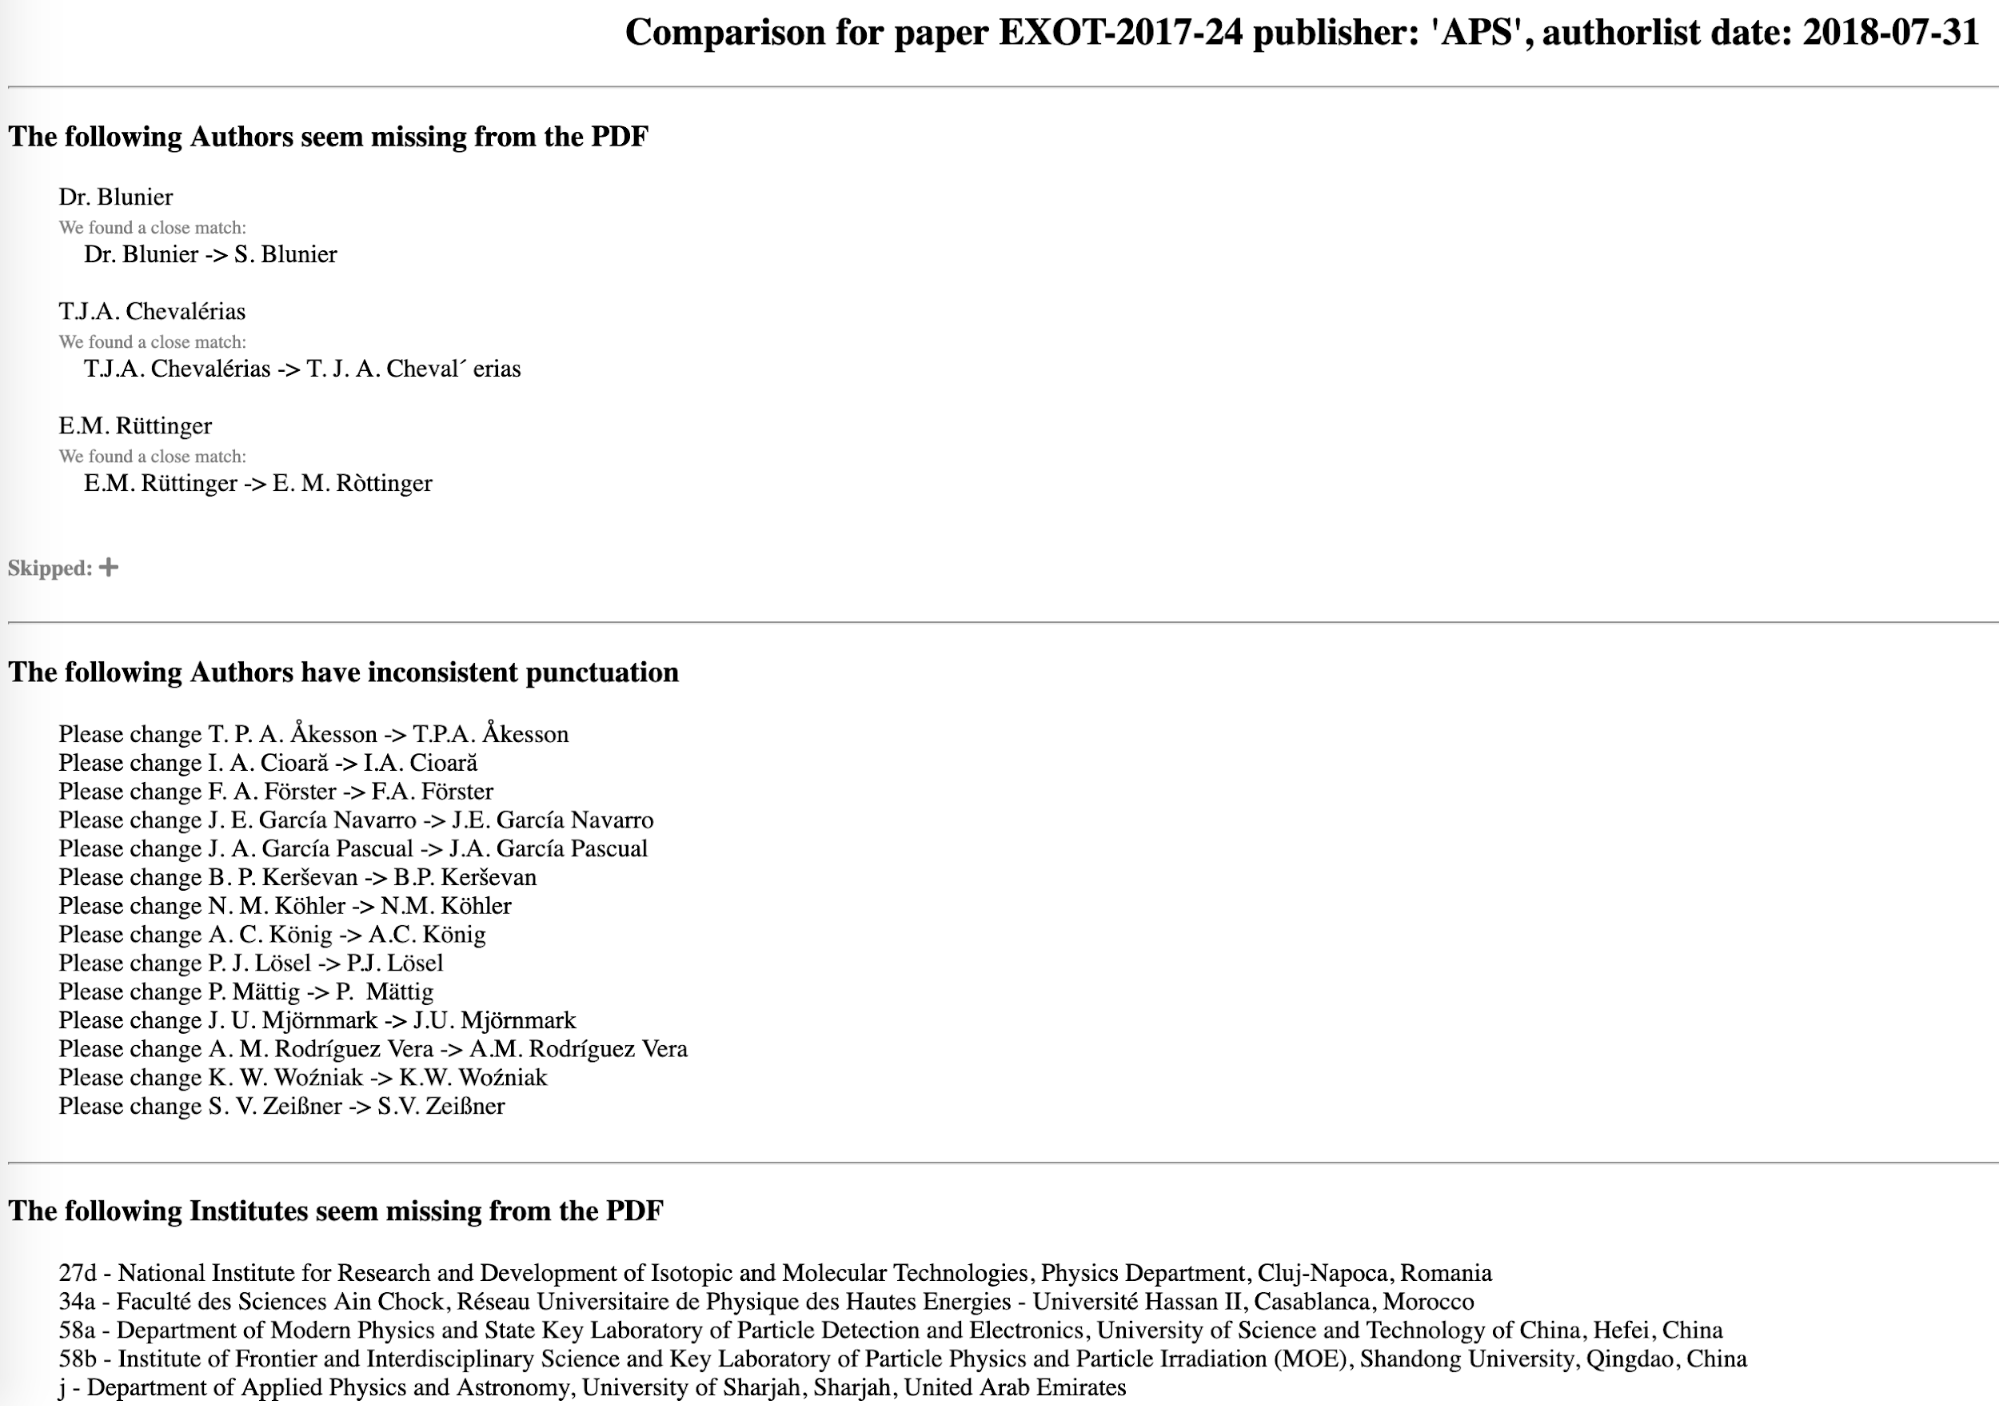
\includegraphics[width=0.9\textwidth]{figures/proof_report_webpage.png}
  \caption{Proof report webpage.}
  \label{fig:proof_report_webpage}
\end{figure}

The proofs checker helps the Physics Office staff in a tedious task, but is far from being a perfect tool.
It needs to be continuously maintained and updated looking for new unexpected cases,
changes in publication layouts, new conventions in the author lists and their format.
A list of further improvements are on the developers agenda,
with the goal of having the user manually check just a couple of dozen cases instead of facing the list of hundreds of false positive they were used to until 2017.
